\documentclass[12pt]{amsart}
\usepackage{amsfonts,amsmath,amsthm,amssymb}
\usepackage[dvipsnames]{xcolor}
\usepackage{tikz}
\usetikzlibrary{matrix}
\usepackage[colorlinks]{hyperref}

\begin{document}

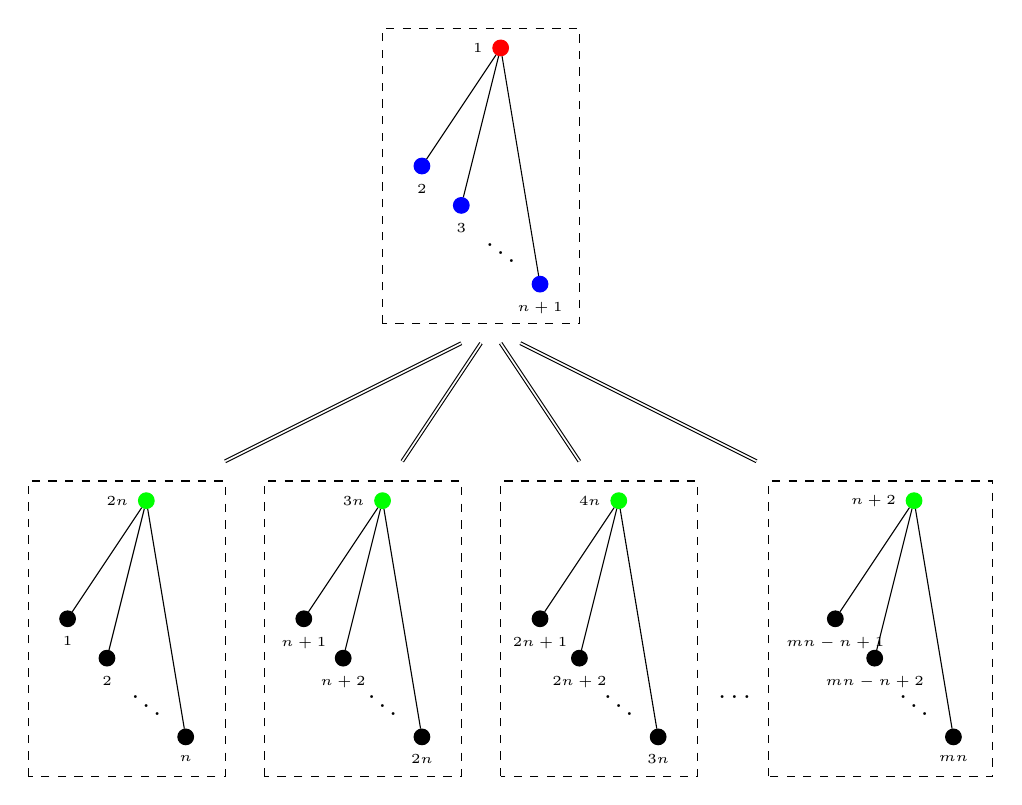
\begin{tikzpicture}[
    scale=0.5,
    every label/.append style={font=\tiny}
]
\tikzstyle{pt}=[draw,shape=circle,inner sep=2pt,fill=black];
% top
\begin{scope}[shift={(6,11.5)}]
    \node[pt,red] (v0) at (2,-1) [label=left:$1$] {};
    \node[pt,blue] (v1) at (0,-4) [label=below:$2$] {};
    \node[pt,blue] (v2) at (1,-5) [label=below:$3$] {};
    \node at (2,-6) {$\ddots$};
    \node[pt,blue] (vm) at (3,-7) [label=below:$n+1$] {};
    \draw (v0) -- (v1) (v0) -- (v2) (v0) -- (vm);
    \draw[dashed] (-1,-8) rectangle (4,-.5);
\end{scope}
% first
\begin{scope}[shift={(-3,0)}]
    \node[pt,green] (v0) at (2,-1) [label=left:$2n$] {};
    \node[pt,black] (v1) at (0,-4) [label=below:$1$] {};
    \node[pt,black] (v2) at (1,-5) [label=below:$2$] {};
    \node at (2,-6) {$\ddots$};
    \node[pt,black] (vm) at (3,-7) [label=below:$n$] {};
    \draw (v0) -- (v1) (v0) -- (v2) (v0) -- (vm);
    \draw[dashed] (-1,-8) rectangle (4,-.5);
\end{scope}
% second
\begin{scope}[shift={(3,0)}]
    \node[pt,green] (v0) at (2,-1) [label=left:$3n$] {};
    \node[pt,black] (v1) at (0,-4) [label=below:$n+1$] {};
    \node[pt,black] (v2) at (1,-5) [label=below:$n+2$] {};
    \node at (2,-6) {$\ddots$};
    \node[pt,black] (vm) at (3,-7) [label=below:$2n$] {};
    \draw (v0) -- (v1) (v0) -- (v2) (v0) -- (vm);
    \draw[dashed] (-1,-8) rectangle (4,-.5);
\end{scope}
% third
\begin{scope}[shift={(9,0)}]
    \node[pt,green] (v0) at (2,-1) [label=left:$4n$] {};
    \node[pt,black] (v1) at (0,-4) [label=below:$2n+1$] {};
    \node[pt,black] (v2) at (1,-5) [label=below:$2n+2$] {};
    \node at (2,-6) {$\ddots$};
    \node[pt,black] (vm) at (3,-7) [label=below:$3n$] {};
    \draw (v0) -- (v1) (v0) -- (v2) (v0) -- (vm);
    \draw[dashed] (-1,-8) rectangle (4,-.5);
\end{scope}
% dots
\node at (14,-6) {$\dots$};
% last
\begin{scope}[shift={(16.5,0)}]
    \node[pt,green] (v0) at (2,-1) [label=left:$n+2$] {};
    \node[pt,black] (v1) at (0,-4) [label=below:$mn-n+1$] {};
    \node[pt,black] (v2) at (1,-5) [label=below:$mn-n+2$] {};
    \node at (2,-6) {$\ddots$};
    \node[pt,black] (vm) at (3,-7) [label=below:$mn$] {};
    \draw (v0) -- (v1) (v0) -- (v2) (v0) -- (vm);
    \draw[dashed] (-1.7,-8) rectangle (4,-.5);
\end{scope}
% double lines
\draw[double] (7,3) -- +(-6,-3) ;
\draw[double] (7.5,3) -- +(-2,-3) ;
\draw[double] (8,3) -- +(2,-3) ;
\draw[double] (8.5,3) -- +(6,-3) ;
\end{tikzpicture}

\end{document}